\section{Proposed System}
\label{sec:system}

Before diving into a description of how the system
is designed and implemented, we first discuss some of our assumptions
about the system and the threat model. Then we will discuss the main
steps involved in searching encrypted data, the initial index generation
and then the actual search process.

\subsection{System Model}

Entities involved in the proposed system are the data owner, CSP and end user.
Data owner is an entity who wants its confidential data to be stored in cloud storage with the capability of privacy-aware searching. 
A cloud service provider (CSP) hosts public cloud storage services for its subscribers on 
a pay-as-you-use model. The end user is an entity who will perform searches on the 
encrypted data stored on the cloud server. The end user can submit search queries 
to the CSP, which evaluates the queries and returns results back to the user. 
Meanwhile during query evaluation, CSP should not be able to learn anything about the query, stored 
data and matching results.

\subsection{Threat Model}

The data owner and end user are considered as trusted entities while CSP 
is considered as a untrusted entity because it is maintained by an 
arbitrary third party. Data communication between end user and CSP should 
be considered as non-trusted as all requests are routed via the open Internet. 
The CSP hosts the encrypted data file ($\mathcal{F}$) and the encrypted index ($\mathcal{I}$). 
As they are encrypted, the CSP cannot learn any information regarding $\mathcal{F}$ and $\mathcal{I}$. 
Query evaluation is done by CSP homomorphically: that is, the CSP performs 
evaluation over encrypted text of $\mathcal{I}$ and encrypted user query, 
so it is neither able to learn anything about the matched results, nor
can it relate any subsequent queries from other users. 


\begin{table*}[t!]
\begin{center}\begin{tabular}{{ |l |l |l }}
    \hline
    Notation & Description\\
    \hline\hline
\vspace*{\fill}\centering $\mathcal{F}$ & Confidential file that needs to
     be outsourced \\\hline
\vspace*{\fill} \centering $\mathcal{K}\omega$ & List of keywords in a data file
$\mathcal{F}$ \\\hline \vspace*{\fill} \centering $f\omega$ & Frequency of a keyword $k\omega$ \\\hline
\vspace*{\fill} \centering $\mathcal{L}$ & Allowed keyword length for extraction
of list of keywords from data \\\hline
\vspace*{\fill} \centering $\mathcal{I}$ & Index file having encrypted bloom filter for each keyword, frequency and number of 1ns as index entries \\\hline
\vspace*{\fill} \centering $\mathcal{E}_h$ , $\mathcal{D}_h$
     & Homomorphic encryption and decryption functions \\\hline
\vspace*{\fill} \centering$\mathcal{E}_S$ , $\mathcal{D}_S$ & Symmetric
    encryption and decryption functions \\\hline
\vspace*{\fill} \centering $\sigma_{pk}$ , $\sigma_{sk}$ & Homomorphic
    encryption public and private keys \\\hline
\vspace*{\fill} \centering$\mathcal{K}_S$ & Symmetric encryption and
    decryption keys. It is used to encrypt the data file. \\\hline
\vspace*{\fill} \centering$\mathcal{S}_q$ & Similarity score of a query
\\\hline
\vspace*{\fill} \centering$\mathcal{R}_q$ & Compressed resultant term after bloom filter matching
\\\hline
\vspace*{\fill} \centering$\mathcal{M}_q$ & Uncompressed resultant term after bloom filter matching
\\\hline
\vspace*{\fill} \centering $\mathcal{O}_b$ & Number of 1ns in a bloom filter
\\\hline
\end{tabular}
\end{center}
\caption{ Notations used in mathematical and descriptive details  }
\label{tab:notations}
\end{table*}


\subsection{Assumptions and Notations}

We ignore key exchange mechanism between the data owner, CSP and the end user, assuming
that it happens using secure out-of-band channels.
Table \ref{tab:notations} illustrates the notations that we use in order to explain
the details of our proposed approach.


\subsection{Index Generation}

The data owner generates an encrypted index on the client side to facilitate
subsequent searches. At a high level, the index is generated by creating a 
\textit{sliding window bloom filter} which is then encrypted using the Pascal Paillier
homomorphic encryption algorithm~\cite{pascal}. 

The sliding window bloom filter (SWBF) is a special type of bloom filter
for which a window size is defined, and based on that
window size, a keyword is mapped to the bloom filter. For example, suppose we have a word
\emph{cloud} and \emph {window size = 2}. Now \emph{cloud} will be sliced into
\emph{cl}, \emph{lo}, \emph{ou}, and \emph{ud} and each of these slices will be 
independently mapped to the bloom filter. This filter enables us to achieve
 a high matching score even if the requested keyword does not match completely.

\begin{algorithm}
\KwIn{A collection of text files $C = \langle \mathcal{F}_1, \mathcal{F}_2, \ldots,
\mathcal{F}_n \rangle$}
\KwOut{Index files $I = \langle \mathcal{I}_1, \mathcal{I}_2, \ldots,
\mathcal{I}_n \rangle$ for each text file  in $C$}
$ \forall \mathcal{F}_i \in \langle \mathcal{F}_1, \mathcal{F}_2, \ldots,
\mathcal{F}_n \rangle$\;
\While{$\mathcal{F}_i \in  C $}{
  $\mathcal{K}\omega \gets extractAllKeywords (\mathcal{F}_i)$\;
  $\forall k\omega_i \in \mathcal{K}\omega $\;
          \While{$k\omega_i \in \mathcal{K}\omega$}{
            $SBF \gets createSWBF (k\omega_i)$\;
            $f_i \gets getKeywordFrequency (k\omega_i) $\;
                $\mathcal{O}_b \gets getOnes (\mathcal{BF}_i) $\;
            $\forall bf_i \in SBF $\;
                \While{$bf_i \in SBF$}{
                        $\mathcal{BF}_i \gets \mathcal{E}_h (\sigma_{pk}, bf_i) $\;
                        $IndexEntry \gets IndexEntry,\mathcal{BF}_i $\;
                        $bf_i \gets getNextBit (SBF) $\;
                }
                $IndexEntry \gets IndexEntry,f_i, \mathcal{O}_b $\;
                $\mathcal{I}_i \gets writeToIndexFile (IndexEntry) $\;
                $k\omega_i \gets getNextKeyword (\mathcal{K}) $\;
          }
  $\mathcal{F}_i \gets getNextFile (C) $\;
}
\Return{$\mathcal{I}_i$}\;
 \caption{Index Creation}
 \label{algo:IndexCreation}
\end{algorithm}

Algorithm~\ref{algo:IndexCreation} describes the indexing procedure.
For each file to be uploaded to the server, a separate index file is generated. The index
file contains one index entry per keyword. To generate the index file, a sliding window bloom
filter is updated for each keyword and the number of 1 bits in the bloom filter are noted.
Each bit of the bloom filter is then encrypted using the Pascal Paillier algorithm, and written to 
the index entry along with frequency and number of 1 bits.
At the end of this process, each index entry $\mathcal{I}_i$ in an index file $\mathcal{I}$ has
the structure: 
\begin{equation}
\mathcal{I}_i = \mathcal{BF}_1,\mathcal{BF}_2, \ldots ,\mathcal{BF}_n, f\omega,
\mathcal{O}_b
  \label{eq: indexEntry}
\end{equation} 
where $\mathcal{O}_b$ is the number of 1's in the bloom filter.

Once the encrypted index file has been generated, it is uploaded to the cloud along with the data files.
The data files are encrypted using a symmetric encryption algorithm, as they will not be used during the
search process.

\subsection{Search Process}

To start the search process, the user first generates a query through a similar process as index creation. 
Each of the user's specified keywords are used to generate sliding window bloom filters, whose bits are then
encrypted using the public key $\sigma_{pk}$ of the Pascal Paillier algorithm. 
Note that this process takes place on the end user's machine. After encryption, 
the query (comprising the encrypted bloom filters) is sent to the cloud for terms matching.

On receiving a query, the CSP will match the incoming query with the index entries of 
the files it is hosting. For a perfect match, all of the corresponding bits of the index 
and query bloom filters need to match. However, since both the query and the index
bloom filters are encrypted, simple matching is not possible. Furthermore, encrypting the
same plaintext repeatedly results in completely different ciphertexts, which improves
privacy and security but makes matching difficult.

Fortunately, homomorphic encryption provides a way to perform mathematical operations 
over ciphertext. Since our bloom filter entries are encrypted using Pascal Paillier homomorphic
encryption, we can just multiply their ciphertexts, which when decrypted, would yield the sum of
the plaintexts~\cite{pascal}. The sum of the bits will be either $0$,$1$ or $2$ after decryption.
The twos in the decrypted output then represent the matched
bits and the ones represent the unmatched bits. Then, a measure of the similarity
can be estimated as the ratio of twos to ones in the decrypted result.

Note that decryption of this result will require users to have the private Pascal 
Paillier key. Thus only authorized users who have received the private key from the
data owner can actually decrypt the results.

\subsection{Compressing Search Results}

Once the encrypted index entries and query have been added together, 
we can simply return their sums back to the client. The client can then decrypt the
sums and compute similarity scores. While this straightforward approach works and
is used by many existing systems for example in~\cite{zeehan}, it is extremely
inefficient.
In particular, if there are many documents and keywords in the cloud dataset, this
will result in a huge amount of data to be communicated back to the user. In quantitative terms,
the summed index entry for \textit{all} keywords in the dataset will be returned
to the client. This will not only increase the response time over the network, but
also the cost of cloud computing for the data owner, since network usage is billed
by most cloud service providers.

In order to reduce this communication cost overhead, we devised a method by which
we are able to reduce this cost by over $95\%$. Based on the insight that each returned
index entry consists only of $0$s, $1$s or $2$s, we
define a polynomial $\mathcal{P}$ given by Equation \ref{eq: polynomial}. 
\begin{equation}
\mathcal{P} = 3^0\cdot\mathcal{BF}_1 + 3^1\cdot\mathcal{BF}_2 +
3^2\cdot\mathcal{BF}_3 + \ldots + 3^{n-1}\cdot\mathcal{BF}_n
  \label{eq: polynomial}
\end{equation}
where $\mathcal{BF}_i$  are the Paillier sums of the corresponding bits
of an index entry and represent variables for
the polynomial $\mathcal{P}$ and $\mathcal{BF}_i \in \langle 0,1,2 \rangle $.

The sum of this polynomial $\mathcal{P}$ is the resultant compressed term which we return back
to client application:

\begin{equation}
\mathcal{R}_q = \sum_{i=0}^{n-1} 3^{i}\cdot\mathcal{BF}_i
\label{eq:compressed}
\end{equation}

From Eq.\ref{eq:compressed} we get a single compressed term $\mathcal{R}_q$ and its size will be
the size of Pascal Paillier key size. This multiplication by constants and addition is again possible 
because our bloom filter entries are encrypted using Pascal Paillier homomorphic
encryption. Therefore, if after decryption, we want the product of the plaintext with a constant, we
just need to exponentiate the ciphertext by that constant~\cite{pascal}.

This means that irrespective of the size
of the bloom filter,
we will always return a single number back to the client. The client can then
decompress it to find out the original Paillier sums using the routine
specified in Algorithm \ref{algo:decomp}. In short, this algorithm works correctly because every
$\mathcal{BF}_i$ is at most 2 and $ 3^{n} > 2\sum_{j=0}^{n-1} 3^{j}$ . This means
that taking $log_3 \mathcal{R}_q$ repeatedly will yield the position of the next
bloom filter entry that needs to be incremented.

\begin{algorithm}
\KwIn{A compressed index entry $\mathcal{R}_q$}
\KwOut{Matched result $\mathcal{M}_q$ comprising a sequence of 0s, 1s and 2s}
$ b \gets 3 $ \;
$i \gets 0 $\;
\While{$\mathcal{R}_q > 0$}{
  $i \gets \log_b \mathcal{R}_q$ \;
  $\mathcal{R}_q \gets \mathcal{R}_q - b^{i}$ \;
  $\mathcal{M}_q [i] \gets \mathcal{M}_q [i] + 1 $ \;
}\Return{$\mathcal{M}_q$}\;
 \caption{Index entry decompression}
 \label{algo:decomp}
\end{algorithm}

The savings achieved using this algorithm can be evaluated using a simple theoretical
formulation. Suppose we use a 32-bit bloom filter and a $64$-bit Pascal Paillier key.
Then for 1000 keywords, the data owner will create an index file with 1000 entries.
Then the size of the index file will be $32*64*1000/8 = 256KB$. On the other hand,
after compression, the number returned per keyword will just have a size equal to the
size of the Paillier key, namely 64 bits. So the total data returned will be 
$64*1000/8 = 8KB$, a saving of over 95\%.


\section{Results}
\label{sec:eval}
We choose a real cloud environment. Google cloud ecosystem, to demonstrated the
viability of our proposed scheme. We implement an indexer, a searching and a
client application as standard Java services. Searching application is deployed
on Google App Engine configured as F4 class instance with a 2.4 GHz CPU and 512
MB of RAM. We utilized Google Blobstore for hosting of index files. We preferred
Blobstore over datastore as datastore has certain limitations like it’s one
entity can hold only few bytes of data and with the increase index entries it’s
read/write operations can be more costly while in Blobstore we can store our complete index file and can access it in searching application so it provides more scalability.
We evaluate the results of our approach on a dataset of 150 documents. 
These documents range in size from 5 MB to 100 MB, containing from 5000 to
129,000 keywords. The keywords were chosen to be at least 8 characters in
length and Porter stemming~\cite{porter} was applied to those keywords.
The client was a Lenovo Thinkpad 430 with a 2.6 GHz Intel Core(TM) i5-332M
CPU and 8 GB of RAM.

\subsection{Indexing Performance}
Figure \ref{fig:Index-Generation-Time} shows execution time for the index creation
and encryption 
processes over different input dataset sizes 
using a 64-bit Pascal Paillier key and a 3 KB bloom filter. The graph shows that
both encryption and index creation sizes increase linearly with input dataset size.

\begin{figure}[h!]
  \centering
  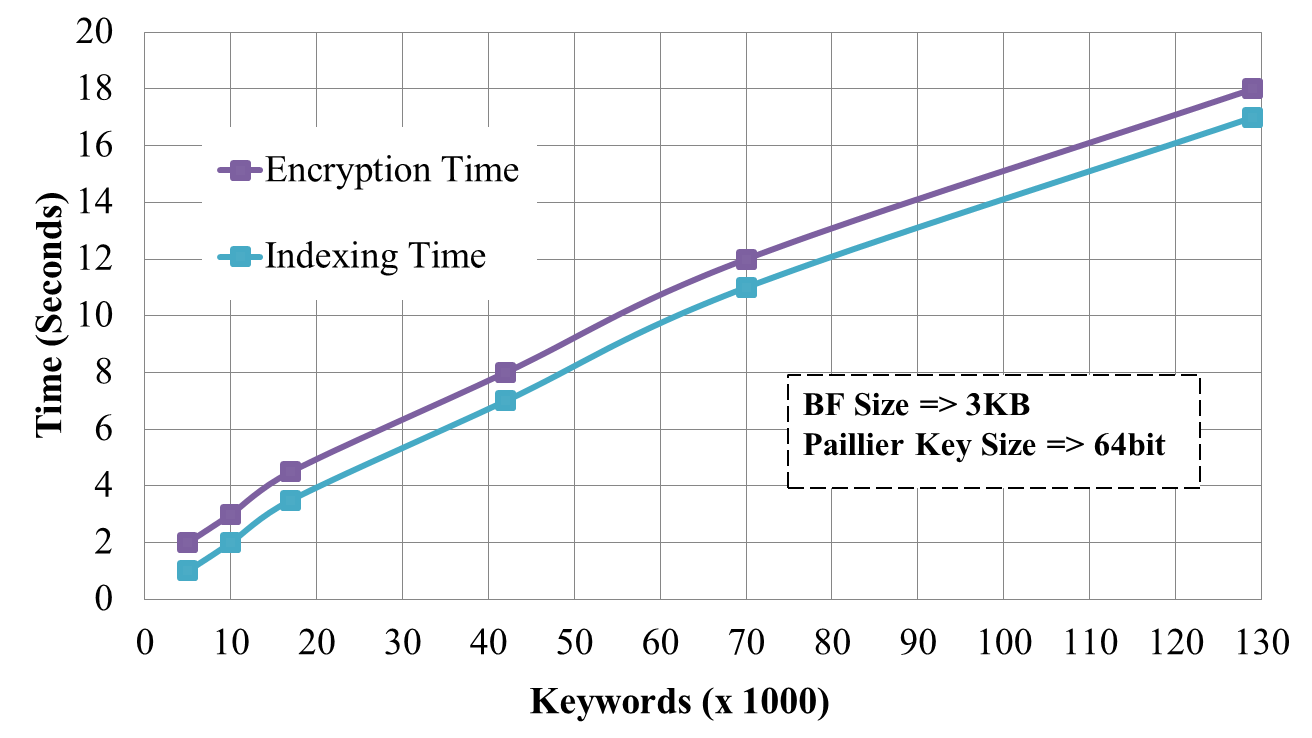
\includegraphics[width=3.5in]{figures/indexing_encryption_time.png}
  \caption{Index Generation Time}
  \label{fig:Index-Generation-Time}
\end{figure}

Paillier key size and bloom filter size both have a substantial impact on index file size. 
With the increase of bloom filter size, the size of each
index entry will increase, which will result in a larger overall index file
size. The increase in indexing time with increasing bloom filter size 
is shown in Figure \ref{fig: bf-size-exe-time}

 \begin{figure}
  \centering
  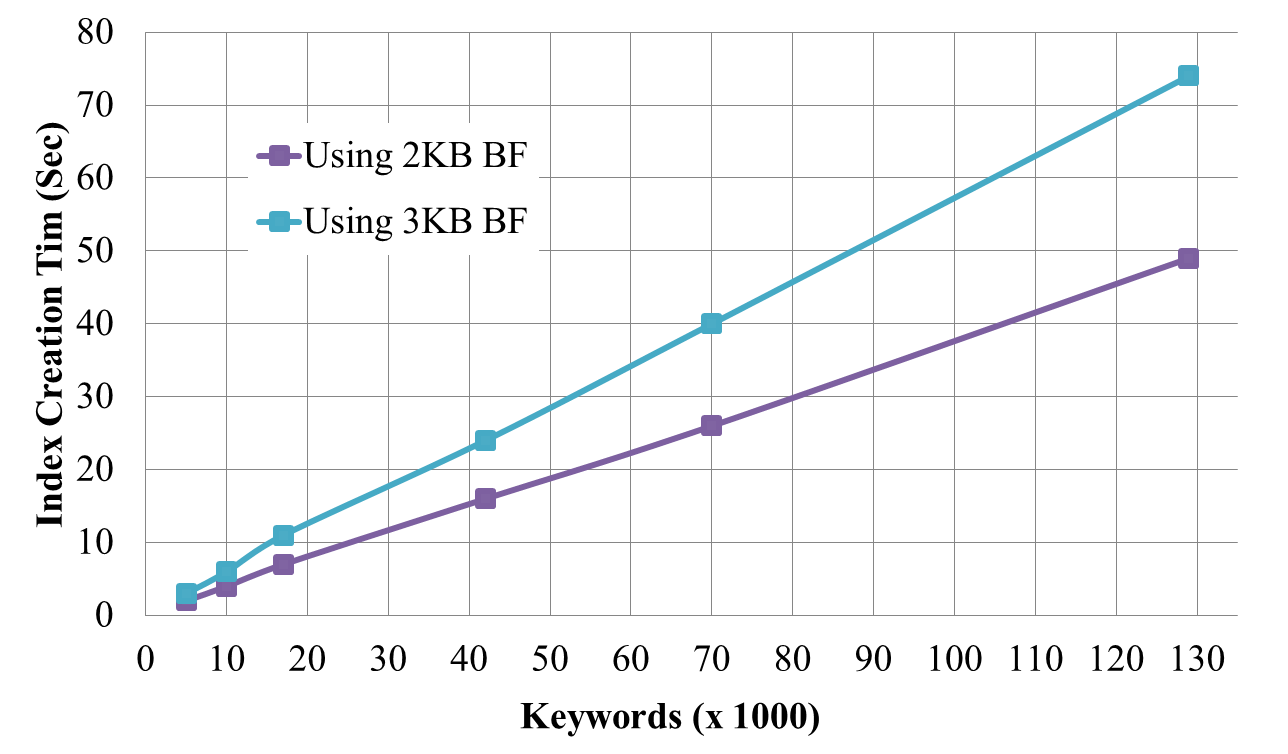
\includegraphics[width= 3in]{figures/index_time_graph.png}
  \caption{Impact of Bloom Filter size on index generation time}
  \label{fig: bf-size-exe-time}
\end{figure}

A larger Paillier key size can help strengthen system security. However, with
increasing Paillier key size, index file size also increases proportionally,
as shown in
Figure \ref{fig: pascal-size-exe-time}.

 \begin{figure}
  \centering
  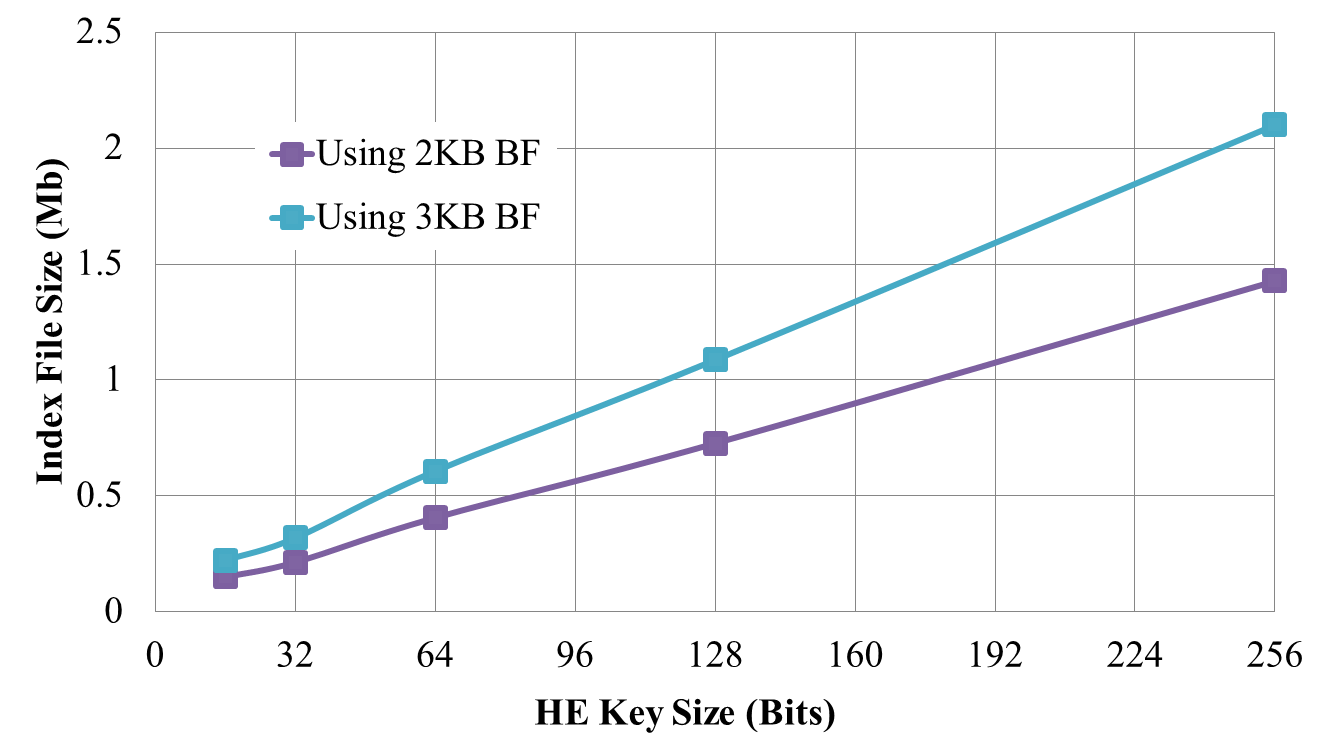
\includegraphics[width= 3in]{figures/paillier_index_size_graph.png}
  \caption{Paillier Key Size Impact on Index File Size}
  \label{fig: pascal-size-exe-time}
\end{figure}

\subsection{Search Performance}

Search performance is evaluated in terms of data returned by a query, response
time, CPU cycles used to process a search request and the cost(\$) CSP will
charge for search queries. 
For private term matching and data returned, our implementation demonstrates
that by using our compression algorithm, data returned to the client
is 95\% less than traditional approaches and remains constant even when the size
of the bloom filter increases. This is shown in Figure \ref{fig:compress}.

\begin{figure}[h!]
  \centering
  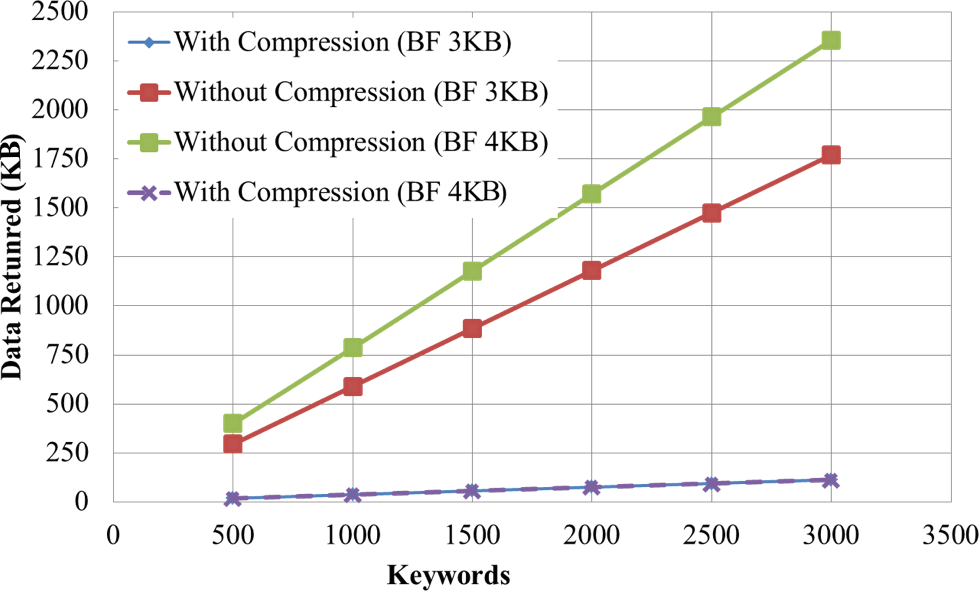
\includegraphics[width= 3.5in]{figures/comp_compare.png}
  \caption{Data returned by a search query: compressed vs uncompressed results}
  \label{fig:compress}
\end{figure}

We also measure the time it takes to extract the matching bloom filter values
from the compressed responses.
Table \ref{tab:search_response_time} show the results. As expected, 
the extraction time increases linearly with the keyword count
on the server.

\begin{table}[th!]
\centering
\begin{tabular}{| c | c | }
\hline
Keyword Count & Response Extraction Time (ms) \\
\hline
500  &  60 \\
1000 &  125 \\
1500 &  185 \\
2000 &  250 \\
2500 &  310 \\
3000 &  370 \\
\hline
\end{tabular}
\caption{Response time increases almost linearly with keyword count.}
\label{tab:search_response_time}

\end{table}


\subsection{Cost Estimation and Response Times}

Finally, we evaluate the cost(\$) that CSP will charge to data owners for search
queries. Our results, shown in Figure \ref{fig:cost_single_query}, demonstrate that a query
searching for a single keyword in a dataset having 500-3500 index entries will cost only \$0.000002 to \$0.00002 per 1000 similar
queries. Furthermore, all of these metrics increase linearly with number of index entries.
We obtained this cost from Google App Engine logs for each data point. In
each log entry \emph{ms}, \emph{cpu\_ms} and \emph{cpm\_usd} depicts the wallclock response
time for a request, the \emph{normalized} CPU time needed to process the
request, and cost(\$) incurred for 1000 similar requests~\cite{google_cloud_logs}.


\begin{figure}
  \centering
  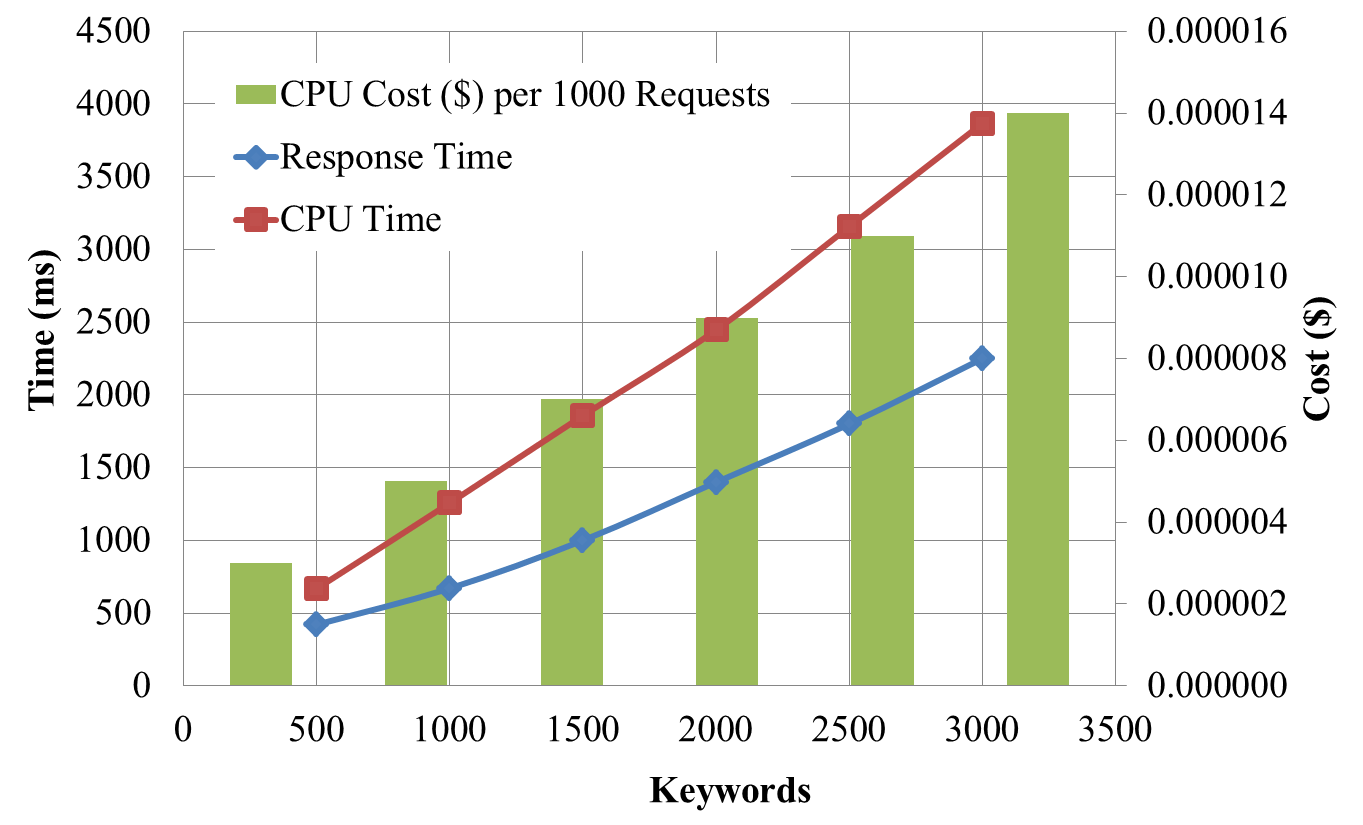
\includegraphics[width= 3.6in]{figures/cost_keywords_graph.png}
  \caption{Searching Cost(\$) with Single Keyword Query}
  \label{fig:cost_single_query}
\end{figure}
